% -%-%-%-%-%-%-%-%-%-%-%-%-%-%-%-%-%-%-%-%-%-%-%-%-%
% MDI224 % 
% Data:12/12/2011                                 %
% Paris,France                                    % 
% Groupe:                                         %
% - Tiago Chedraoui Silva                   % 
% - Anthony CLERBOUT
% -%-%-%-%-%-%-%-%-%-%-%-%-%-%-%-%-%-%-%-%-%-%-%-%-%

\documentclass[a4paper,11pt]{article}

\usepackage[francais,listings,algo]{tcs}

% Cover %
\def \ttprofname{Roland BADEAU} % teachers name
\def \ttabrv{MDI224} % abbreviation of names class
\def \ttabrvxt{} % period
\def \mytitle{Interpolation par splines cubiques} % Big title
\def \mysubtitle{ Travaux Pratique 2 - Deuxième semestre de 2011} % subtitle
\def \ttauthi{Anthony CLERBOUT} % author's name
\def \ttxti{Casier: 234} % Extra text right side of name
\def \ttauthii{Tiago CHEDRAUOI SILVA} % author's name
\def \ttxtii{Casier: 214 } % Extra text right side of name
\def \ttdate{Décembre 15, 2011} % date

\begin{document}
\titleTMB 
\newpage
\tableofcontents
\listoffigures
\newpage

\section{Résolution du système linéaire}

\subsection{Méthode du gradient à pas constant}

\subsubsection{Implémentation}

Pour voir la méthode du gradient à pas constant, on a fait le code suivant:

\begin{multicols}{2}
  \lstinputlisting[title=\textbf{Méthode du gradient à pas constant}]{../mygradient.m}
\end{multicols}

Losqu'on l'utilise, on trouve comme solution:

\begin{center}
$x = [ 0.99996 \; 1.00002 \; 0.99998 \; 1.00002 \; 0.99996]^T$
\end{center}

Cette solution n'est pas optimal, mais est beaucoup proché de la solution opimal
($x^* = [ 1.0 \; 1.0 \; 1.0 \; 1.0 \; 1.0]^T$
);

\subsubsection{Variation du taux de convergence}

\begin{figure}[h!]
  \begin{centering}
    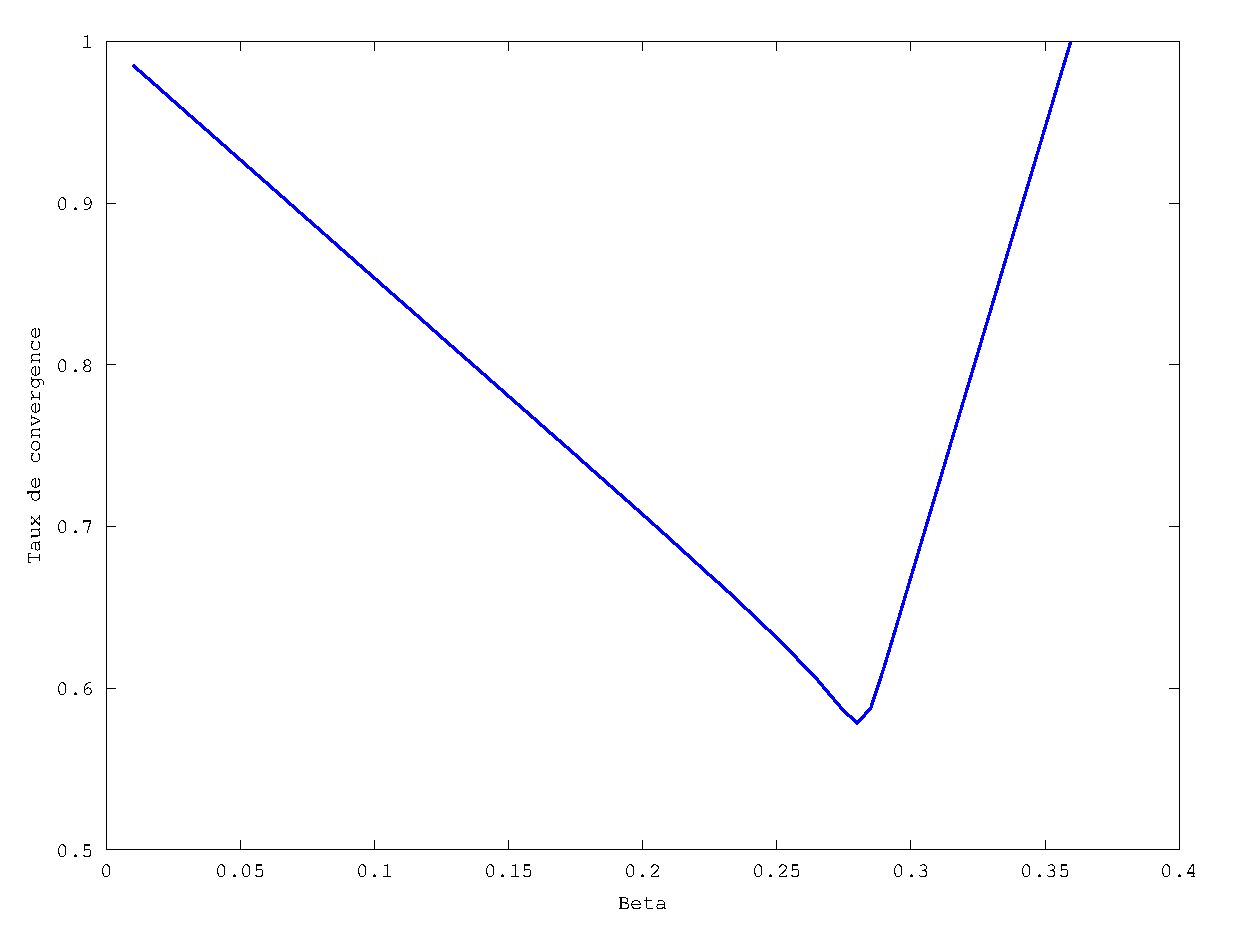
\includegraphics[scale=0.5]{../grad_beta}
    \label{rspro2}
    \par\end{centering}
  \caption{Taux de convergence de la méthode gradient en fonction de beta}
  \label{fig:jacobi-conv}
\end{figure}

\newpage
\subsection{Méthode du gradient à pas optimal}

\subsubsection{$\beta$ qui minimise $J(x_k)-\beta g_k$}

Pour trouver $\beta$ qui minimise $J(x_k)-\beta g_k$,
avec $g_{k+1}=-\nabla J(x_k+\beta_kg_k)$.

Soit:
\begin{eqnarray*}
f'(\beta_k)= 0 &=& (\nabla J(x^k+\beta_kg_k),g_k)\\
&=&-(g_{k+1},g_k)=-g_{k+1}^Tg_k
\end{eqnarray*}

On a $g_{k+1}= b -Ax_k-\beta_kAg_k=g_k-\beta_kAg_k$

Donc :
\begin{eqnarray*}
 (g_{k+1},g_k) = 0  &\Rightarrow&  (g_k-\beta_kAg_k,g_k)  = 0\\
   & \Leftrightarrow& (g_{k},g_k)-\beta_k(Ag_k,g_k) = 0\\
  & \Leftrightarrow&  \beta_k=\frac{(g_{k},g_k)}{(Ag_k,g_k)}= \frac{(g_{k}^T,g_k)}{g_k^TA^Tg_k}
\end{eqnarray*}


\subsubsection{Implémentation}
Pour voir la méthode du gradient à pas optimal, on a fait le code suivant:

\begin{multicols}{2}
  \lstinputlisting[title=\textbf{Méthode du gradient à pas optimal}]{../gradient_optimal.m}
\end{multicols}


\subsubsection{Taux de convergence}
\begin{figure}[h!]
  \begin{centering}
    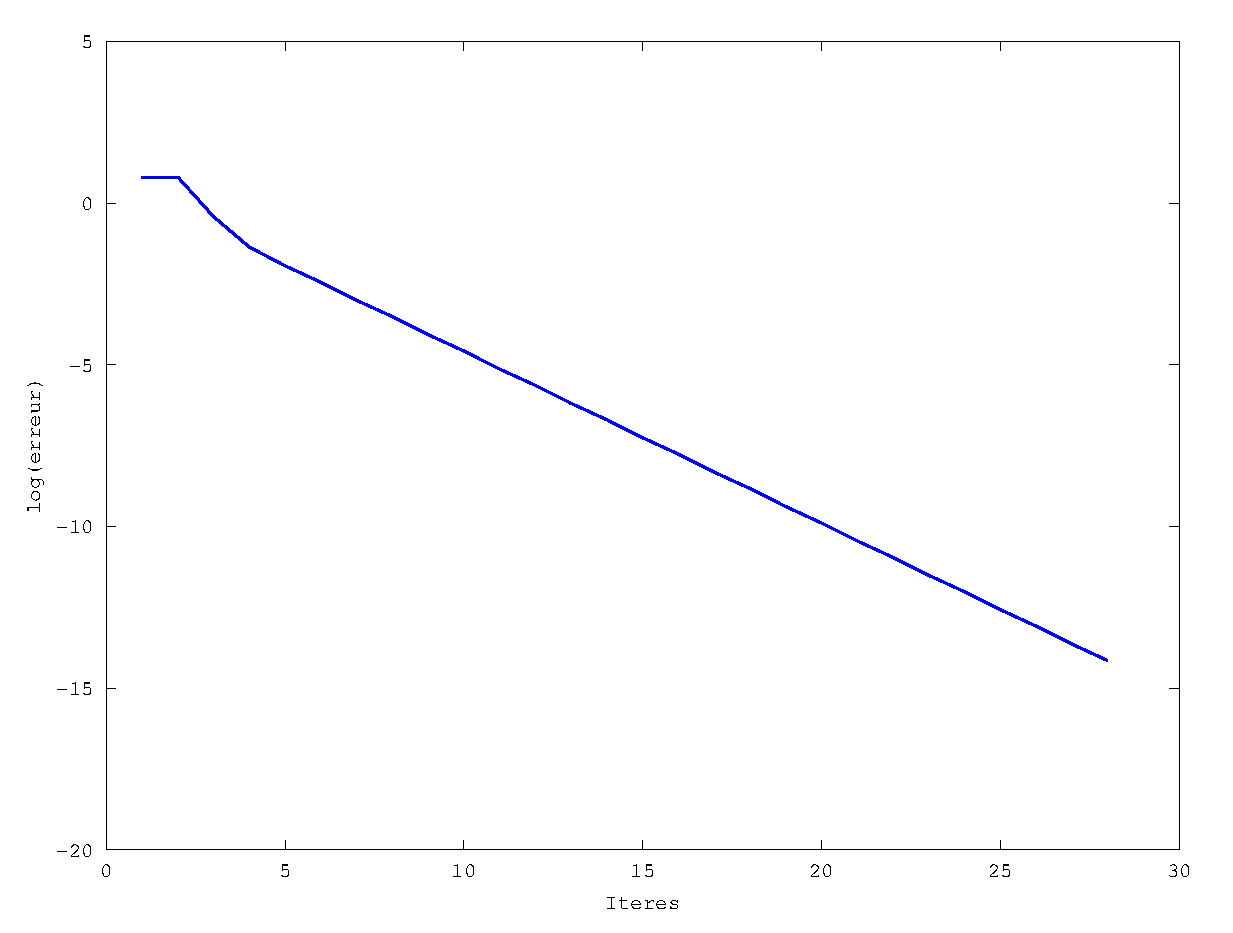
\includegraphics[scale=0.5]{../grad_optimal}
    \label{rspro2}
    \par\end{centering}
  \caption{Convergence de la méthode gradient optimal}
  \label{fig:jacobi-conv}
\end{figure}

En utilisant la fonction polyfit de Matlab, on a trouvé $\text{p(x)= -0.547007 x
  + 1.029611 }$. Donc, le taux de convergence de
l’algorithme trouvée est: -0.54.

\subsection{Méthode du gradient conjugué}
\subsubsection{Implémentation}

Pour voir la méthode du gradient conjuge, on a fait le code suivant:
 
\begin{multicols}{2}
  \lstinputlisting[title=\textbf{Méthode du gradient conjugué}]{../gradient_conjugue.m}
\end{multicols}

\subsubsection{Complexité}
Le nombre de iteration de cet algorithme est proportionelle à la taille n de la matrice du système, cela veut dire que le gradient conjugué converge en au plus n itérations.
Pour une matrice  pleine la méthode demande $2n^3$  opérations, comme la matrice
est creuse, le méthode fera moins que $2n^3$  opérations.

\subsubsection{Temps d'exécution}

\begin{table}[h!]
  \begin{center}
    \begin{tabular}{|c|c|}
      \hline 
      Méthode & Temps \\
      \hline 
      \hline 
      Gradient conjugué & 0.0017250 s\\
      Relaxation & 0.0044890\\
      Gradient optimal & 0.0044729 s\\
      \hline 
    \end{tabular}
  \end{center}
  \caption{Comparatif de les temps de exécution de différentes méthodes de
    résolution linéaire}
\end{table}


\section{Application }

\begin{multicols}{2}
  \lstinputlisting[title=\textbf{Calcul de spline cubique naturelle}]{../tstinvtridiag0.m}
\end{multicols}



\begin{figure}[h!]
  \begin{centering}
    \subfigure[Example 1]{
      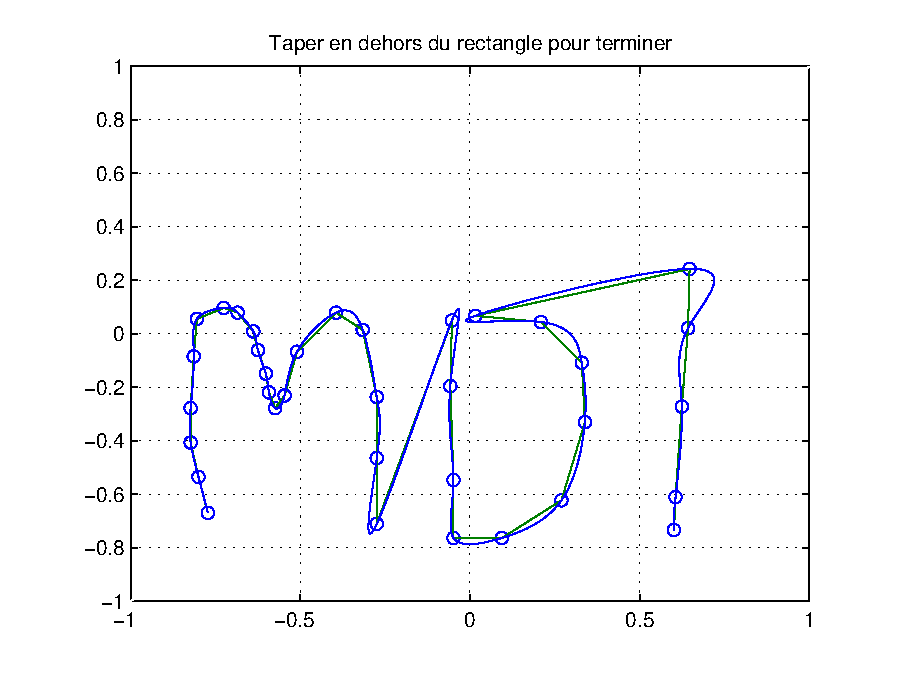
\includegraphics[scale=0.35]{../figue_spline3}}  
    \subfigure[Example 2]{
      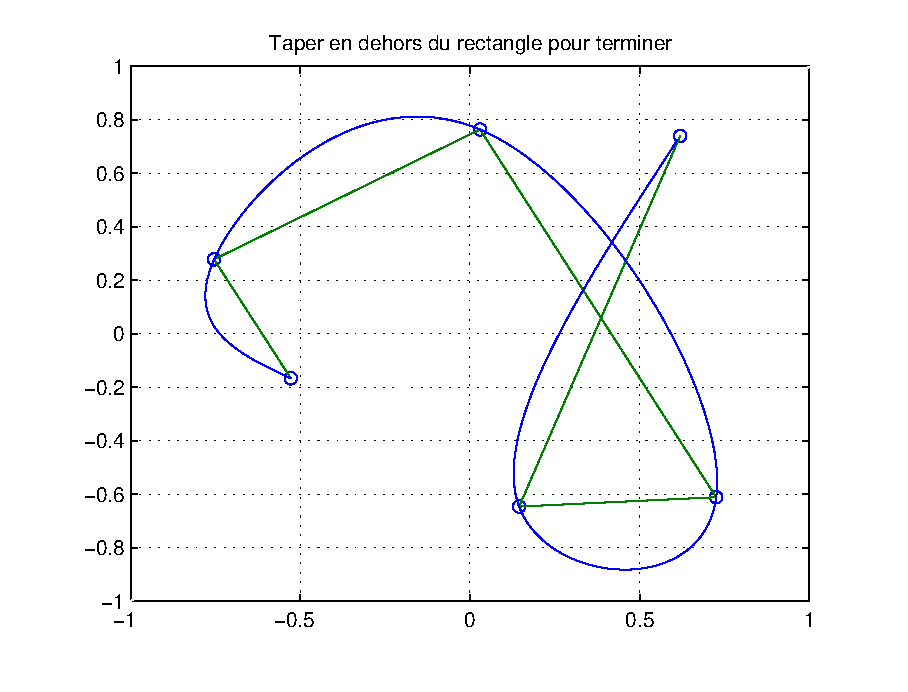
\includegraphics[scale=0.35]{../exemple_spline_naturelle}
    }
    \par\end{centering}
  \caption{Calcul de spline cubique naturelle}
  \label{rspro}
\end{figure}

\end{document}

